\section{Data and experiments}
\label{sec:experiments}
%
\subsection{Shape prior}
%
As described in \autoref{sec:introduction}, the general situation in
the connectivity pipelines consists of having 
a reliable segmentation obtained from the high resolution \gls{t1} 
reference image. Therefore, a precise location of the tissue interfaces
of interest is available in a reference space. Given that the anatomical 
reference segmentation is beyond the scope of this manuscript, we simply 
rely on the true contours known from the underlying models, and do not 
seek to establish them in a separate segmentation step on ``anatomical'' images.
%
\subsection{Synthetic gray-scale data}
%
The first simplified model to test the approach is inspired by a problem 
shown for coupled \gls{csf}/\gls{gm} and \gls{gm}/\gls{wm} segmentation in \citep{macdonald_automated_2000}. Authors note that ``partial volume effects 
blur the distinction between closely adjacent surfaces in deep sulci, leading 
to a well-known segmentation error in which the deeper reaches of sulci are 
not penetrated by the putative surface model.'' This problem is aggravated 
in DWI, since the resolution tends to be worse compared to the anatomical 
images considered in \citep{macdonald_automated_2000}. They test their 
coupled segmentation algorithm on an image, ``representing a sulcus in 
which the distinction between opposing banks of the sulcus has been obscured 
by partial volume.''  

Here, we reproduce their model on a volume consisting of three 
piecewise-constant parts: a notched ball representing the \gls{wm} with a single 
sulcus ($\mu_{WM} = 0.8$), a cortical sheet of \gls{gm} obtained through dilation 
of the \gls{wm} ($\mu_{GM} = 0.5$), and the surrounding background representing 
\gls{csf} ($\mu_{CSF} = 0.2$). The volume is then affected by additive Gaussian 
noise, effectively creating uniform standard deviation of $\sigma = 0.045$ per 
region.

As illustrated in \autoref{fig:sulcusmodel}, conventional single surface 
segmentation of the \gls{csf}/\gls{gm} boundary misses to capture the sulcus in 
its full depth. With our proposed model, we expect the joint 
segmentation-registration to be driven largely by the inner, \gls{gm}/\gls{wm}
contour that exhibits sufficient contrast and lesser partial volume effects. 
The shape prior of the outer, difficult contour will then be co-aligned through 
the regularity of the estimated deformation field.

\begin{figure}
\begin{tabular}{ccccc}
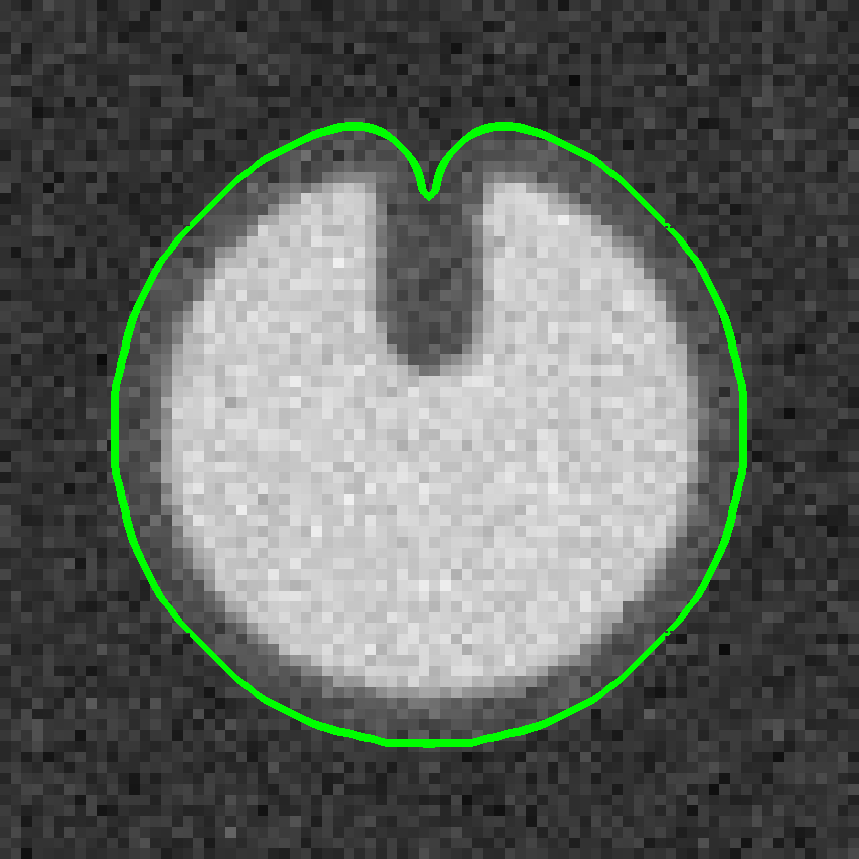
\includegraphics[width=0.19\textwidth]{contours_wrong} & 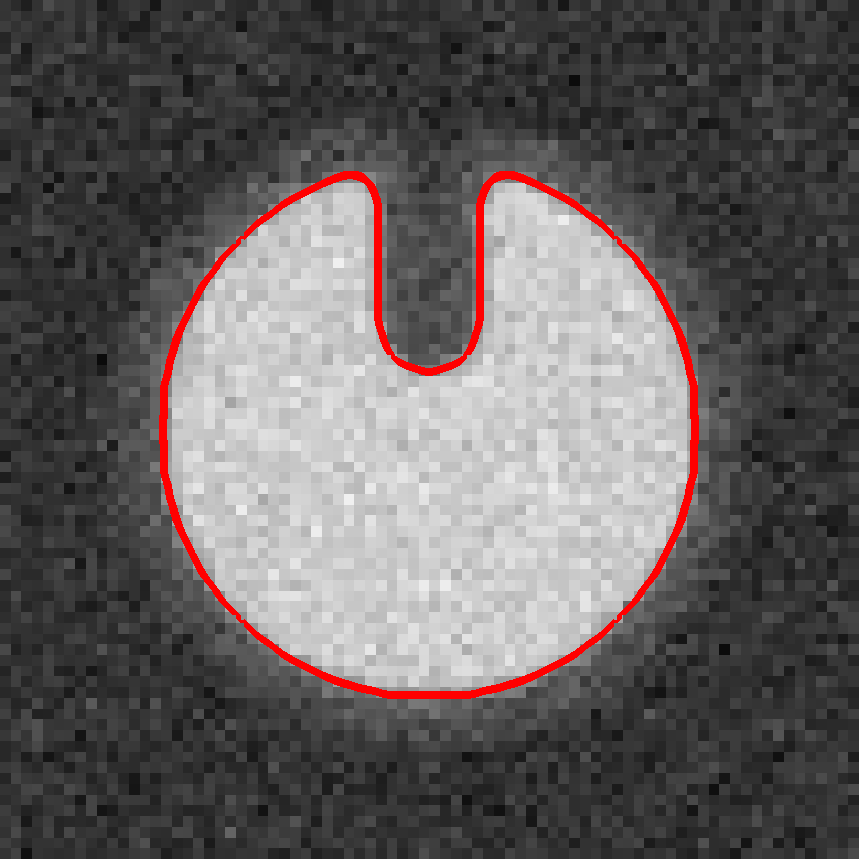
\includegraphics[width=0.19\textwidth]{contours_inner} &
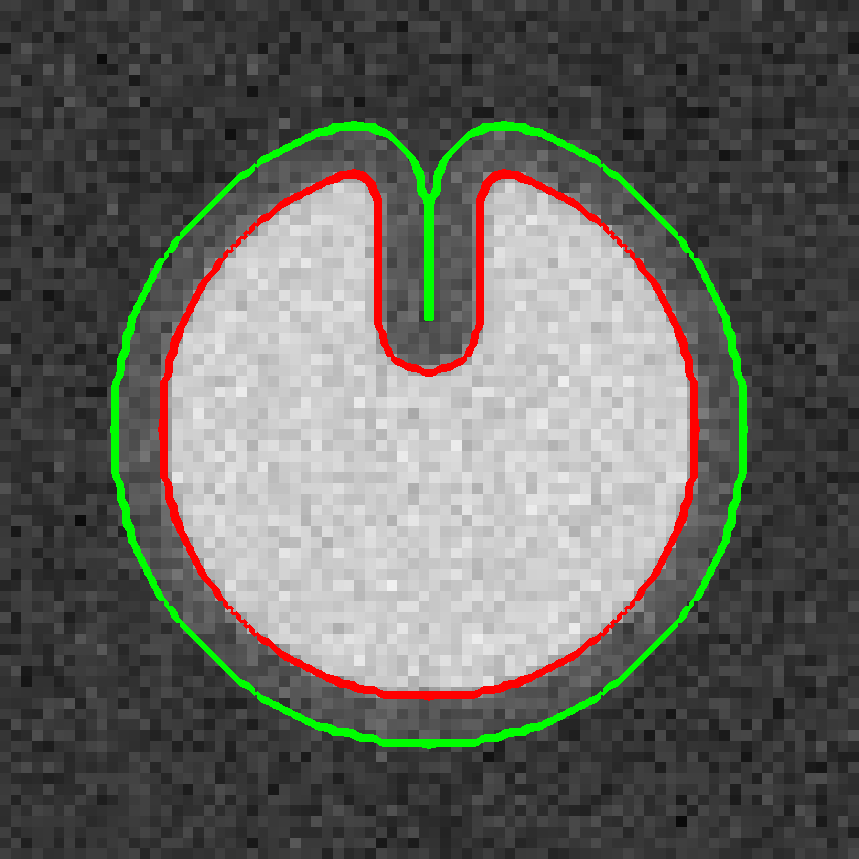
\includegraphics[width=0.19\textwidth]{contours_both} &
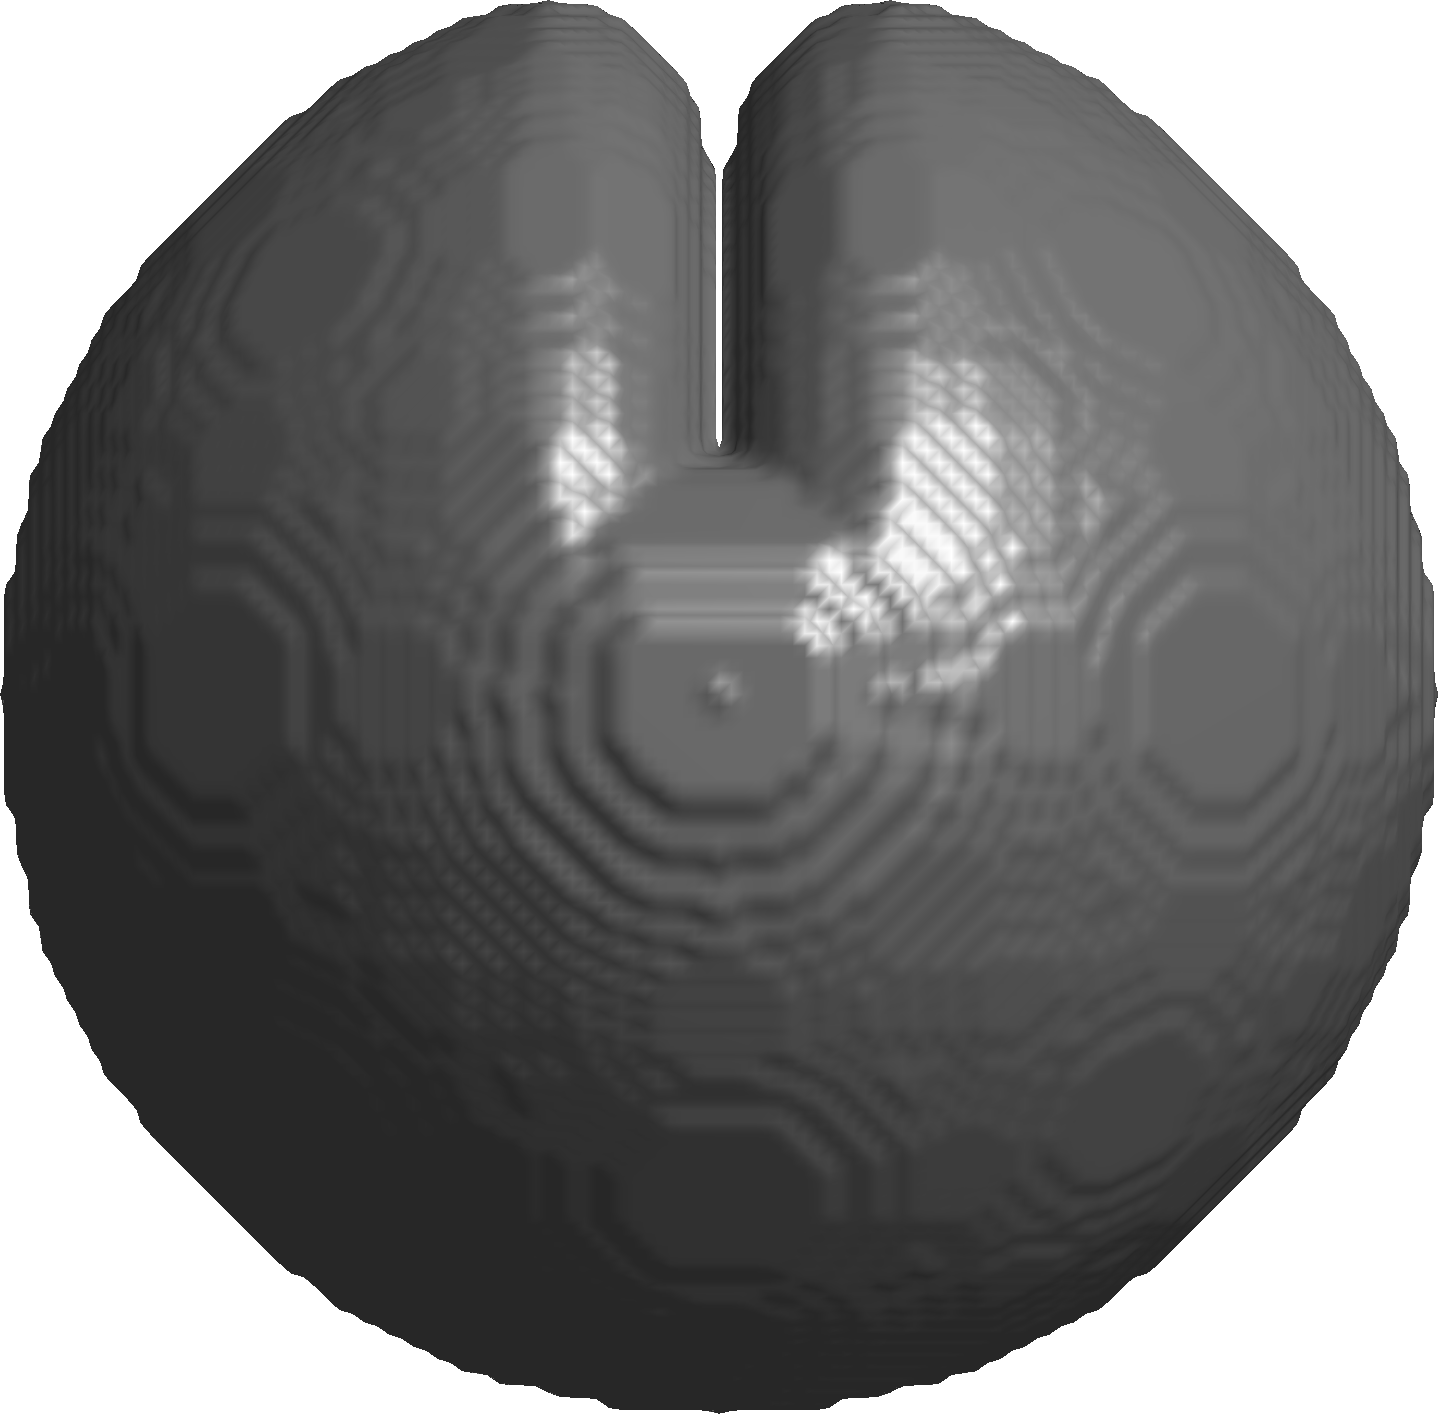
\includegraphics[width=0.19\textwidth]{pialsurf} &
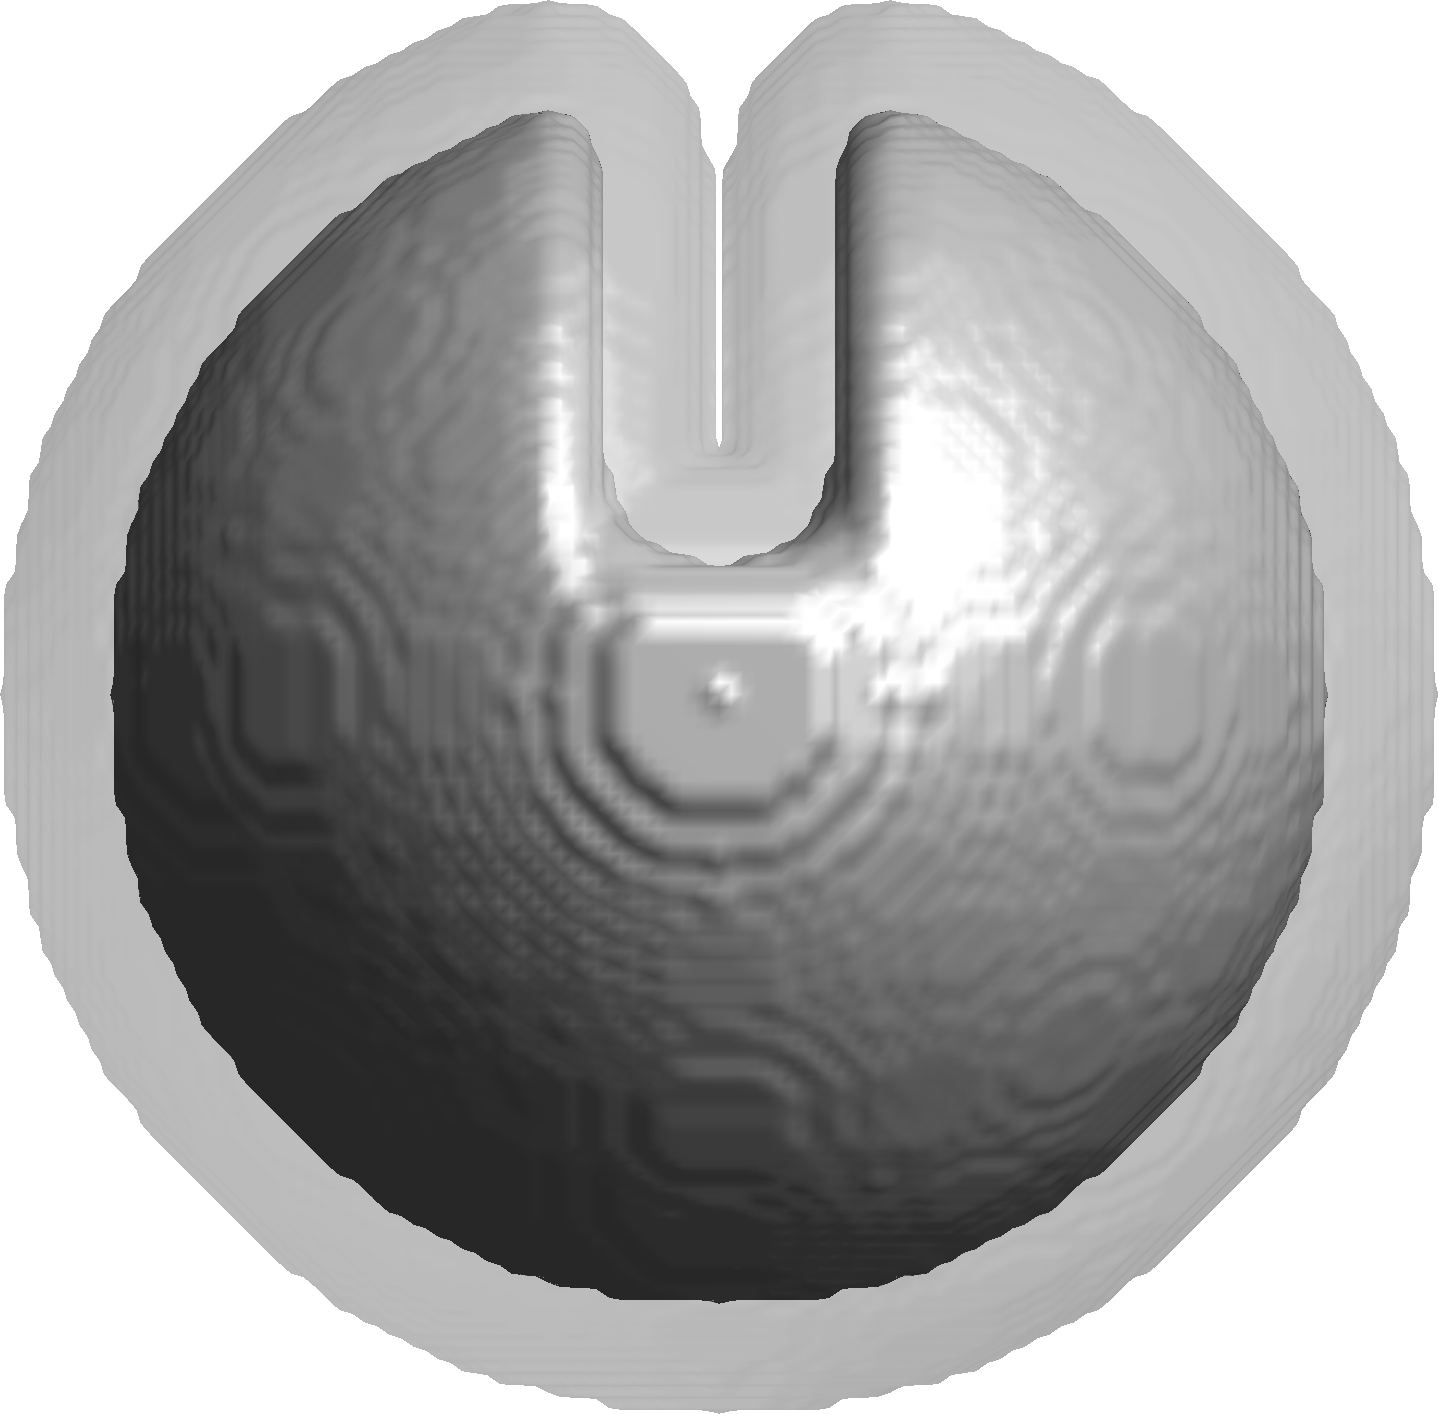
\includegraphics[width=0.19\textwidth]{gmwmsurf}\\
a)&b)&c)&d)&e)
\end{tabular}
\caption{The gray-scale sulcus model. a) The apparent CSF/GM boundary is affected by partial volume in the sulcal cavity, and conventional segmentation is likely to miss it. b) The GM/WM interface here has consistently good contrast. c) Registering the two shape priors coupled through deformation field regularity is expected to guide the CSF/GM contour. d\&e) 3D view of the two shape priors.}
\label{fig:sulcusmodel}
\end{figure}



%
\subsection{Simulated diffusion data}
%
In order to demonstrate the functionality of the methodology, 
and characterize its possibilities with diffusion data,
we built a synthetic phantom from a model consisting of several 
spherical shapes emulating the different brain tissues (see 
\autoref{fig:fa}, first row). We simulated a single-shell
acquisition at $b=1000$ \eqref{eqn:MultiTensor} with 30 samples
equally distributed on one hemisphere, corresponding to a standard
\gls{dti} acquisition commonly used in clinical practice.
We generated a synthetic displacement field to produce
an \gls{epi}-like distortion on the \gls{dwi} signal. Finally,
we reconstructed the deformed signal, and generated \gls{dwi}-derived
scalar maps (specifically the \gls{fa} and \gls{md} maps).
Then, the scalar maps were placed as features in 
\eqref{eq:complete_energy} to drive our segmentation approach, 
finding the location of the \gls{wm}-\gls{gm}
and the \gls{csf}-\gls{wm} interfaces in the distorted space. \\

\paragraph{Signal simulation}
To numerically simulate the \gls{mri} signal attenuation when applying a diffusion 
gradient in a voxel with $N$ fiber populations we made use of the standard 
\emph{Multi-Tensor Model}~\cite{Tuch:2002aa}:
%
\begin{equation} 
\label{eqn:MultiTensor}
S(q) / S_{0} = \sum_{i=1}^{N} f_{i} \, \exp{ \left( -b \, q^{T} \, \mathbf{D}_i \, q\right) } + f_{iso} \, \exp{ \left( -b \, \mathbf{D}_{iso} \right) }  + f_{gm} \, \exp{ \left( -b \, \mathbf{D}_{gm} \right) } ,
\end{equation}
%
where $q \in \mathbb{S}^2$ is the direction of the diffusion gradient applied,
$b$ is the b-value accounting for its strength and $S_0 \equiv S(0)$ is the 
signal with no diffusion weighting. $f_i$ and $\mathbf{D}_i$ are the volume 
fraction and the diffusion tensor characterizing the $i$-th fiber population, 
whereas the tensors $\mathbf{D}_{iso}$ and $\mathbf{D}_{gm}$ describe the 
diffusion processes of partial volumes with \gls{csf} and \gls{gm} within the 
voxel, which volume fractions are, respectively, $f_{iso}$ and $f_{gm}$, and
$\sum_i f_i + f_{iso} + f_{gm} = 1$. In this work, the diffusion properties have
been taken from standard ranges typically observed in the human 
brain~\cite{Canales-Rodriguez:2009aa}. Moreover we assumed $N = 1$ and $S_0 = 1$ 
without loss of generality.

\paragraph{Noise simulation}
The diffusion MRI signal $S$ has been corrupted with 
\textit{Rician noise}~\cite{Gudbjartsson:1995aa} as follows:
%
\begin{equation}
	\tilde{S} = \sqrt{ (S + \varepsilon_1)^2 + \varepsilon_2^2 }
\end{equation}
%
where $\varepsilon_{1,2}$ are Gaussian distributed with zero mean
and standard deviation $\sigma = S_0 / \mathit{SNR}$ and \gls{snr}
is the \gls{snr} on the $S_0$ image.

\paragraph{Simulated \gls{epi} distortion}
For this model, we created manually a sound distortion to approximate
the real \gls{epi} distortions. We interpolated the distortion to a 
dense deformation field, and applied it to generate the deformed \gls{dwi}
signal.

\paragraph{Derived scalar features}
We obtained the local fiber configuration in each voxel with a commonly 
used \gls{dti} reconstruction tool~\footnote{DTIFIT, included
in the FMRIB's Software Library (FSL), 
\url{http://fsl.fmrib.ox.ac.uk/fsl/fsl-4.1.9/fdt/fdt_dtifit.html}}. 
The properties of the reconstructed tensors and derived scalar maps have
been studied by \cite{ennis_orthogonal_2006}. Based on their
findings, \gls{fa}~\eqref{eq:fa} and \gls{md}~\eqref{eq:md} are
considered complementary features, and therefore we selected them for the 
energy model \eqref{eq:complete_energy} in driving the 
registration-segmentation process. 
Whereas \gls{fa} informs mainly about the \emph{shape} of diffusion, 
the \gls{md} is more related to the \emph{magnitude} of the process:

\begin{align}
\mathrm{FA} &= \sqrt{ \frac{1}{2}}\,\frac{\sqrt{ (\lambda_1 - \lambda_2)^2 + (\lambda_2 - \lambda_3)^2 + (\lambda_3 - \lambda_1)^2}}{\sqrt{ {\lambda_1}^2 + {\lambda_2}^2 + {\lambda_3}^2}} \label{eq:fa} \\
\mathrm{MD} &= ( \lambda_1 + \lambda_2 + \lambda_3 ) / 3 \label{eq:md}
\end{align}
where $\lambda_i$ are the eigenvalues of the diffusion tensor 
associated with the diffusion signal $S(\vec{q})$. There exist 
two main reasons to justify their choice. 
First, they are well-understood and standardized in clinical routine.
Second, together they contain most of the information that is
usually extracted from the \gls{dwi}-derived scalar maps
\cite{ennis_orthogonal_2006}. The different region properties 
$(\mathbf{\mu}_R,\Sigma_R)$ measured for the \gls{fa} and \gls{md}
joint distribution are summarized in \autoref{table:parameters}. \\ 

\begin{table}
\caption{Model means and covariances of \gls{fa} and \gls{md} estimated 
from the reconstructed simulated \gls{dwi} images for each modeled tissue, 
\gls{wm}, \gls{gm}, and \gls{csf}. As expected, the two scalar features 
are complementary and the three tissues can well be discriminated. }
\label{table:parameters}
%\begin{tabularx}{1.0\textwidth}{c|XXX}
\begin{tabular}{*{3}{@{}p{0.2\textwidth}}@{}p{0.4\textwidth}@{}}
\toprule
% tissue        & $\mathbf{\mu}_{FA}$ & $\mathbf{\mu}_{MD}$ & $\Sigma$ \newline
        & $\mathbf{\mu}$ \\
\cmidrule(r){2-3}
Tissue& FA & MD &$\Sigma$\\
\cmidrule(r){1-1}\cmidrule(r){2-2}\cmidrule(r){3-3}\cmidrule{4-4}
\gls{wm}  & 0.778 & 6.94\e{-4} & 
   $\begin{pmatrix}
   	4.85\e{-3} & -6.90\e{-6} \\ -6.90\e{-6} & 1.03\e{-8}
   \end{pmatrix}$\vspace{2mm}\\
%
\gls{gm}  & 0.119 & 8.95\e{-4} &
   $\begin{pmatrix}
   	5.90\e{-4} & -1.43\e{-6} \\ -1.43\e{-6} & 1.04\e{-8}
   \end{pmatrix}$\vspace{2mm}
\\
%
\gls{csf} & 0.103 & 2.99\e{-3} &
   $\begin{pmatrix}
   	1.19\e{-3} & 2.22\e{-7} \\ 2.22\e{-7} & 1.56\e{-8}
   \end{pmatrix}$
\\
\bottomrule
\end{tabular}
%\end{tabularx}

\end{table}
